This survey has treated diagnostics and infrastructure as two bodies of work and, in \S\ref{sec:tension}, as two sets of requirements acting on the same runtime objects. This section discusses why the two developed separately, where the field disagrees with itself, what remains unsolved, and what a research agenda grounded in the tension would look like.

\paragraph*{Why the two layers were studied separately.}
The separation is largely sociological rather than technical. Diagnostics draws on two communities that rarely meet: the software engineering fault-localization and testing community (ICSE, ASE, FSE), where the unit of analysis is an execution trace, and the machine-learning community that publishes at ICLR, ICML, NeurIPS, and ACL. In our own reference set the ML side dominates, with only a minority of diagnostic papers (for example FALAT, AgentRx, and MASPrism) appearing at software-engineering venues. Neither community publishes at systems venues, which is where the serving work lives. Infrastructure grew out of systems and architecture (OSDI, SOSP, MLSys), where the unit is a request and the goal is throughput and latency under a resource budget. The two communities show little overlap in our own bibliography. This is an observation about the surveyed set, not a measured co-citation count: none of the serving systems in \S\ref{sec:infrastructure} evaluates against a diagnostic benchmark, and among the failure-localization methods in \S\ref{sec:diag_fl} the three paradigms matured with minimal cross-citation. The budgets differ too: a diagnostics paper can afford twenty replays per failure because it runs offline on a fixed corpus, while a serving paper treats any per-request overhead above single-digit percentages as unacceptable. This is why the tension we identified is not visible from within either community: each has optimized against a constraint the other does not face.

\paragraph*{Contested questions.}
Several genuine disagreements cut across the literature, and our evidence bears on each.

\emph{Should attribution be statistical, reasoning-based, or learned?} The three paradigms in \S\ref{sec:diag_fl} embody different bets. Statistical approaches assume failures leave a reproducible signature across replays; reasoning-based approaches assume a sufficiently capable model can infer the cause from a single trace; learned approaches assume the mapping is stable enough to be trained. The paradigms developed independently, which is either a healthy division of labour, with different regimes favouring different methods, or a duplication problem, in which three communities solve the same task with incompatible evaluation. Our evidence is equivocal. The paradigms do report on overlapping benchmarks now (Who\&When recurs across the statistical, reasoning, and learned families), which suggests convergence is beginning; but they still disagree about what an acceptable input cost is, so their headline numbers are not commensurable. We regard this as an open question rather than a settled one.

\emph{Should trace richness be maximized or minimized?} Diagnostics wants richer traces: TraceElephant's central result is that observability materially changes what can be attributed, with step-level accuracy far more sensitive than agent-level~\citep{traceelephant2026}. Serving wants cheaper traces: the same paper's output-only setting is not a failure of instrumentation but the natural consequence of capturing only what is cheap to keep. Both positions are defensible, and the field has not agreed on where the line sits. The absence of a standard for \emph{what must be retained} (as opposed to what may be captured) is the clearest symptom.

\emph{Is retention an engineering detail or an architectural resource?} Current systems treat retention as a local policy: an eviction rule inside a serving engine, a TTL chosen per workload. Under this framing, diagnostics is simply a consumer that must cope with whatever survives. The alternative, which we favour and which \S\ref{sec:tension} argues for, is that retention is a first-class resource shared between layers, with an explicit budget and explicit trade-offs. Nothing in the current literature settles this; no system reports retention as a managed quantity.

\emph{Should safety intervene proactively or reactively?} The safety paradigms in \S\ref{sec:diag_safety} disagree about when a guardrail should act. Topology-based and policy-verification methods examine a proposed action before it executes; reactive and recovery-oriented methods intervene after detection. The disagreement is substantive rather than stylistic, because the two positions have opposite implications for the tension. A proactive guardrail must hold enough state about the proposed action to judge it, which means retaining execution context that a serving engine would rather evict; a reactive guardrail tolerates a window during which damage may already have propagated through the communication graph. The literature reports both kinds of system as successful, but not on a common workload with a common overhead budget, so the choice between them remains an empirical question. That the field has not settled it is unsurprising given that, as we noted above, no benchmark measures the serving cost of a guardrail at all.

\paragraph*{The safety layer as a third constraint.}
Safety is often filed under diagnostics, and we have followed that convention in our taxonomy, but the tension analysis suggests it behaves differently from either layer. A guardrail is not a passive consumer of traces, like an attribution method, nor a pure resource manager, like a scheduler. It is a component that must inspect runtime state \emph{and} act on the serving path, which places it under both constraints at once: it needs the retention that diagnostics needs in order to judge an action, and it must meet the latency budget that infrastructure meets in order to act in time. Multi-agent settings sharpen this, because the object a guardrail must reason about is not a single agent's state but the communication graph spanning all of them, the same graph whose maintenance cost a serving system is trying to control. We regard the placement of safety within the two-layer picture as genuinely unsettled: treating it as a subcategory of diagnostics, as the prevailing convention does, may understate the scheduling burden it imposes.

\paragraph*{Fundamental concepts and open problems.}
The organising problem is the retention--discard conflict. Diagnostics needs runtime objects to persist until a failure is explained; serving needs them gone as soon as their reuse probability drops. Two cross-layer mechanisms make the conflict concrete (Table~\ref{tab:tension}): eviction swaps agent state off the fast path at the moment a later diagnosis would need it, and serving retains no environment snapshots, so replay-based attribution must reconstruct them offline. A third instance, TrajAudit's trace compression, shows the same shape within the diagnostic layer itself. A fourth, replay cost, marks where the conflict would become acute for any diagnostic that must run on the serving path.

Framed this way, the open problem is an accounting one. A principled treatment would make retention a budgeted quantity, allocated per agent and per trajectory, priced against serving objectives, and released on a schedule rather than by a local eviction heuristic. No published system does this. The nearest analogues are cache-retention policies, which optimise for reuse probability and therefore systematically discard precisely the low-probability states that post-hoc diagnosis prizes. We note that this framing is a proposal, not a result: it follows from the behaviours we verified in the surveyed systems, but no experiment in the literature tests it directly.

\paragraph*{Research gaps.}
Three gaps follow from the above and are, in our reading, the field's most tractable openings. First, \emph{no benchmark measures diagnostics--infrastructure interaction}. Every benchmark surveyed in \S\ref{sec:diag_bench} evaluates attribution quality on a fixed corpus; none measures attribution quality under a realistic serving policy, nor the serving cost of achieving a given diagnostic fidelity. The interaction is therefore unmeasured in both directions. Second, \emph{no standard specifies what must be retained}. OpenTelemetry conventions~\citep{opentelemetry2026} and structured-logging proposals~\citep{agenttrace2026} standardise capture, not retention, so interoperability breaks exactly when a failure is investigated. Third, \emph{evaluation scale is mismatched}. Diagnostics methods are validated on tens to hundreds of failures (FAMAS: 82; TraceElephant: 220; the largest telemetry study we found: 275 executions~\citep{whenfail2026}), while production systems execute thousands of tasks per hour. Whether the reported accuracies survive that scale is untested, and the retention costs that would be required to make them survive are unreported.

\paragraph*{Evidence and its limits.}
Two methodological choices shape what this survey can claim, and both are recorded here because they bound how the results should be read. The first is the verification strategy described in \S\ref{sec:background}. Its consequence is uneven depth. The failure-localization and infrastructure layers contain the systems we could verify against full text, and they carry the quantitative analysis; the observability and safety layers rest substantially on abstract-level evidence, and we have accordingly described what those systems do without ranking them. Readers should treat the two halves of our taxonomy as carrying different evidential weight, which Table~\ref{tab:obs_safety} and Table~\ref{tab:failure_loc} make visible through their tier and publication-type columns.

The second is the recency of the field. A large fraction of the surveyed work (by our count, roughly two-thirds of the cited systems) appears as preprints without a confirmed venue, and several entries carry 2026 dates. This is a property of a fast-moving area rather than a defect of any individual work, but it bounds our conclusions in a specific way: venue-independent claims, such as the existence of the retention--discard conflict, are robust to it, whereas any statement about which method currently performs best is not, because the ranking can change between preprint revisions. We have therefore avoided ranking language throughout and reported matched comparisons only where the source supports them.

\paragraph*{Broader impact.}
The retention question has a privacy dimension that sits alongside its performance dimension. Diagnostics requires retaining execution state, and that state routinely contains user inputs, tool outputs, and reasoning traces; richer retention therefore extends the lifetime of potentially sensitive data. Infrastructure optimisations that predict agent activation introduce a second concern, since an accurate model of when agents will act is also a model of what agents are doing, and could be repurposed for monitoring beyond the operational purpose it was built for. We see no technical mechanism that separates these uses once the state is retained; the practical mitigations are policy-level (bounded retention windows, access control, and audit trails for production deployments~\citep{auditableagents2026}), and they trade away some of the diagnostic fidelity that motivates retention in the first place. This is a genuine cost of the research direction we advocate, and it should be weighed explicitly when retention budgets are designed rather than after the fact.

\paragraph*{Limitations.}
Beyond the evidential asymmetry noted above, five limitations bound this review. First, our infrastructure analysis rests on ScaleSim as a full-text case study, with TokenCake, Continuum, and KAIROS examined at the abstract level; the tension in \S\ref{sec:tension} is argued from the verified behaviour of these components rather than from a purpose-built experiment, and would be strengthened by direct measurement of diagnostic accuracy under real serving policies. Second, the third workload characteristic of contribution~2 (inter-agent memory sharing) is likewise characterised at the abstract level, so the systems cited under it are enumerated rather than compared. Third, the survey lacks a formal search methodology: we did not run a registered protocol with predefined databases, query strings, date windows, or screening criteria, so the system and reference set should be read as a curated landscape rather than as the output of a reproducible search, and a systematic review with PRISMA-style reporting would likely surface additional systems. Fourth, the safety discussion draws on venue-published work (G-Safeguard at ACL, ShieldAgent at ICML) alongside preprints read at abstract level; the former were verified through their published text but without page-level cross-checking of every reported number. Fifth, our taxonomy is descriptive of what has been built, not predictive of what should be: where we identify an absent capability, such as retention accounting, we are reporting a gap in the literature rather than asserting that no unpublished system has closed it. Our verification strategy trades quantitative breadth for citation honesty, and these limitations mark where that trade is most visible. We note that citing preprints does not breach the journal's policy on unpublished material, which concerns unpublished original data rather than public preprints of reviewed work.

\begin{figure*}[t]
\centering
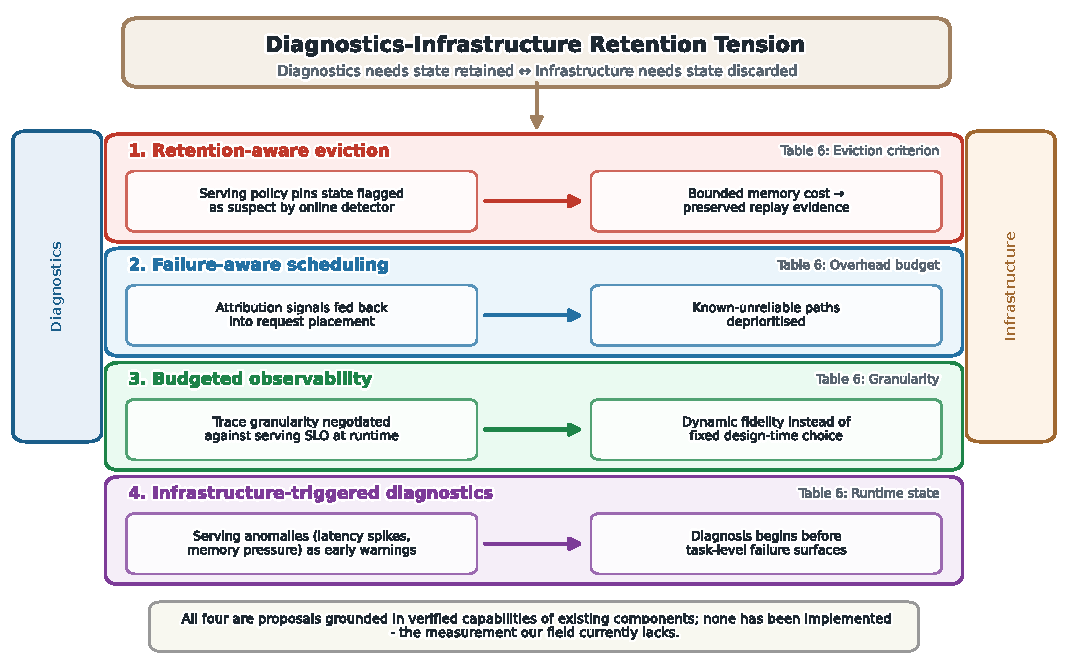
\includegraphics[width=\textwidth]{fig6_codesign_agenda.pdf}
\caption{Co-design research agenda derived from the diagnostics--infrastructure tension. Four directions address specific rows of Table~\ref{tab:tension}: retention-aware eviction, failure-aware scheduling, budgeted observability, and infrastructure-triggered diagnostics. Each converts a tension point into a concrete research challenge at the boundary between the two layers.}
\label{fig:codesign}
\end{figure*}

\paragraph*{Future development.}
The four co-design directions introduced in \S\ref{sec:tension} and developed here form a research agenda rather than a list of features, because each addresses a specific row of Table~\ref{tab:tension}. \emph{Retention-aware eviction} would let a serving policy pin the state that an online detector flags as suspect, converting a bounded memory cost into preserved replay evidence. \emph{Failure-aware scheduling} would feed attribution signals back into request placement, so that known-unreliable execution paths are deprioritised. \emph{Budgeted observability} would negotiate trace granularity against the serving SLO at runtime instead of fixing it at design time. \emph{Infrastructure-triggered diagnostics} would treat serving anomalies such as latency spikes and memory pressure as early-warning signals that begin diagnosis before the task-level failure surfaces. We stress that all four are proposals grounded in the verified capabilities of existing components; none has been implemented, and each would need to demonstrate that the serving cost it incurs is repaid by diagnostic gains, the measurement our field currently lacks.